% Created 2024-05-08 Wed 15:06
% Intended LaTeX compiler: pdflatex
\documentclass[smaller]{beamer}\usepackage{listings}
\usepackage{color}
\usepackage{amsmath}
\usepackage{array}
\usepackage[T1]{fontenc}
\usepackage{natbib}
\lstset{
keywordstyle=\color{blue},
commentstyle=\color{red},stringstyle=\color[rgb]{0,.5,0},
literate={~}{$\sim$}{1},
basicstyle=\ttfamily\small,
columns=fullflexible,
breaklines=true,
breakatwhitespace=false,
numbers=left,
numberstyle=\ttfamily\tiny\color{gray},
stepnumber=1,
numbersep=10pt,
backgroundcolor=\color{white},
tabsize=4,
keepspaces=true,
showspaces=false,
showstringspaces=false,
xleftmargin=.23in,
frame=single,
basewidth={0.5em,0.4em},
}
\usepackage{natbib, dsfont, pgfpages, tikz,amssymb, amsmath,xcolor}
\bibliographystyle{abbrvnat}
\setbeamertemplate{footline}[frame number]
\beamertemplatenavigationsymbolsempty
\usepackage{appendixnumberbeamer}
\setbeamercolor{gray}{bg=white!90!black}
\setbeamertemplate{itemize items}{$\circ$}
\lstset{basicstyle=\ttfamily\footnotesize}
\RequirePackage{fancyvrb}
\DefineVerbatimEnvironment{verbatim}{Verbatim}{fontsize=\footnotesize}
\definecolor{bblue}{rgb}{0.2,0.2,0.7}
\newcommand{\E}{{\ensuremath{\mathop{{\mathbb{E}}}}}}
\newcommand{\R}{\mathbb{R}}
\newcommand{\N}{\mathbb{N}}
\newcommand{\blank}{\makebox[1ex]{\textbf{$\cdot$}}}
\newcommand\independent{\protect\mathpalette{\protect\independenT}{\perp}}
\def\independenT#1#2{\mathrel{\rlap{$#1#2$}\mkern2mu{#1#2}}}
\renewcommand{\phi}{\varphi}
\renewcommand{\epsilon}{\varepsilon}
\newcommand*\diff{\mathop{}\!\mathrm{d}}
\newcommand{\weakly}{\rightsquigarrow}
\newcommand\smallO{\textit{o}}
\newcommand\bigO{\textit{O}}
\newcommand{\midd}{\; \middle|\;}
\newcommand{\1}{\mathds{1}}
\usepackage{ifthen} %% Empirical process with default argument
\newcommand{\G}[2][n]{{\ensuremath{\mathbb{G}_{#1}}{\left[#2\right]}}}
\DeclareMathOperator*{\argmin}{\arg\!\min}
\DeclareMathOperator*{\argmax}{\arg\!\max}
\newcommand{\V}{\mathrm{Var}} % variance
\newcommand{\eqd}{\stackrel{d}{=}} % equality in distribution
\newcommand{\arrow}[1]{\xrightarrow{\; {#1} \;}}
\newcommand{\arrowP}{\xrightarrow{\; P \;}} % convergence in probability
\newcommand{\KL}{\ensuremath{D_{\mathrm{KL}}}}
\newcommand{\leb}{\lambda} % the Lebesgue measure
\DeclareMathOperator{\TT}{\Psi} % target parameter
\newcommand{\empmeas}{\ensuremath{\mathbb{P}_n}} % empirical measure

\renewcommand*\familydefault{\sfdefault}
\itemsep2pt
\usepackage[utf8]{inputenc}
\usepackage[T1]{fontenc}
\usepackage{graphicx}
\usepackage{longtable}
\usepackage{wrapfig}
\usepackage{rotating}
\usepackage[normalem]{ulem}
\usepackage{amsmath}
\usepackage{amssymb}
\usepackage{capt-of}
\usepackage{hyperref}
\usetheme{default}
\author{Anders Munch}
\date{May 8, 2024}
\title{Regularity and adaptive debiased machine learning \newline}
\subtitle{Journal club'ish inspired by \newline \emph{Adaptive debiased machine learning using data-driven model selection techniques} \citep*{van2023adaptive}}
\begin{document}

\maketitle

\begin{frame}[label={sec:org413e683}]{Short experience with \sout{Twitter}}
\begin{center}
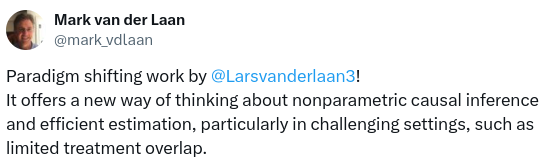
\includegraphics[width=1\textwidth]{./twitter-laan-quote.png}
\end{center}
\end{frame}

\begin{frame}[label={sec:org4582758}]{Motivation}
Build \emph{practically} useful estimators that can be used with high-dimensional
longitudinal register data. Is the targeted learning philosophy sometimes too
much ``asymptopia'' (mathematically correct limit results, but practically
useless)?

\vfill

Understand of regularity.
\end{frame}


\begin{frame}[label={sec:orgb277aa5}]{The targeted learner and the modeler}
\begin{minipage}[t]{.8\linewidth}
  Specify your target parameter and your model. Also pre-specify your estimator.
\end{minipage}
\vfill
\begin{flushright}
  \begin{minipage}[t]{.8\linewidth}
    I don't yet know enough about the data, I need to estimate some models and
    see which fit.
  \end{minipage}
\end{flushright}
\vfill
\begin{minipage}[t]{0.8\linewidth}
  You shouldn't do that, use a super learner to let the computer decide these
  things instead.
\end{minipage}
\vfill
\begin{flushright}
  \begin{minipage}[t]{.8\linewidth}
    I am not sure if that will work in practice. I will start with a simple
    model, and if that looks OK, I will stick with it.
  \end{minipage}
\end{flushright}
\vfill
\begin{minipage}[t]{0.8\linewidth}
  Your approach leads to invalid statistical inference!
\end{minipage}
\vfill
\begin{flushright}
  \begin{minipage}[t]{.8\linewidth}
    Your approach is too likely to lead to enormous CI or even estimates that
    are \texttt{NA}!
  \end{minipage}
\end{flushright}
\end{frame}

\begin{frame}[label={sec:org3881282}]{Acknowledge limitations of ``off the shelf'' TL}

Simple stating that we estimate $\Psi \colon \mathcal{M} \rightarrow \R$ under
a non-parametric model might be too optimistic/simplistic.

\vfill

There can be problems that we had not thought about (e.g., positivity problems
for specific subgroups).

\vfill

For complex data with many variables (e.g., longitudinal register data), we
might not be able to solve this problem well enough for practical sample sizes.

\vfill

It might not be possible to construct an estimator which is valid across the
fully nonparametric model \emph{and} works well in practice for reasonable sample
sizes.
\end{frame}


\begin{frame}[label={sec:org7bba150}]{From the abstract}
\begin{quote} %% Abstract
Debiased machine learning estimators for nonparametric inference of smooth
functionals of the data-generating distribution can suffer from excessive
variability and instability. For this reason, practitioners may resort to
simpler models based on parametric or semiparametric assumptions. However, such
simplifying assumptions may fail to hold, and estimates may then be biased due
to model misspecification. To address this problem, we propose Adaptive Debiased
Machine Learning (ADML) [\ldots{}]. By learning model structure directly from data,
ADML avoids the bias introduced by model misspecification and remains free from
the restrictions of parametric and semiparametric models. [\ldots{}]

\flushright \cite{van2023adaptive}
\end{quote}
\end{frame}


\begin{frame}[label={sec:org4a51930}]{\color{white} breaker}
\huge\centering \color{bblue} Intermezzo on semi-parametric efficiency theory
\end{frame}

\begin{frame}[label={sec:org90acf5a}]{RAL estimators and semi-parametric efficiency theory}

An estimator \( \hat{\Psi}_n \) of $\Psi \colon \mathcal{M} \rightarrow \R$ is
\textit{asymptotically linear} (AL) if for all \( P \in \mathcal{M} \) there
is a function \( \phi(\blank; P) \in \mathcal{L}_P^2 \) with
\( P{[\phi(\blank; P)]}=0 \) such that
\begin{equation*}
  \hat{\Psi}_n - \Psi(P) = \frac{1}{n} \sum_{i=1}^{n} \phi(X_i; P) + \smallO_P{(n^{-1/2})}.
\end{equation*}
The function \( \phi(\blank; P) \) is the \textit{influence function} (IF) of
the estimator.

\vfill

AL estimators can compared by comparing the norm of their IFs. The \emph{efficient
influence function} (EIF) is the IF with smallest norm.

\vfill

Expect that an estimator which has the EIF as its IF is ``optimal'' in some sense.

\vfill

A further regularity condition is needed for this to be true -- the estimator
should be \emph{regular}.
\end{frame}

\begin{frame}[label={sec:org64fb1f6}]{Regularity}
\begin{beamercolorbox}[rounded=true]{gray}

\centering An estimator \( \hat{\Psi}_n \) of
$\Psi \colon \mathcal{M} \rightarrow \R$ is \textit{regular} if its asymptotic
distribution is invariant to local perturbations of the data generating
mechanism.
\end{beamercolorbox}

\begin{block}{}
\small

% Formally: Let \(\mathcal{M} \) be a collection of probability measure and
% $\Psi \colon \mathcal{M} \rightarrow \R$ a parameter of interest.

% \hfill

Formally: A one-dimensional submodel \( \{P_t : t \in \R\} \subset \mathcal{M} \)
through \( P \) at \( t=0 \) is \textit{regular} if it is differentiable in
quadratic mean at \( t=0 \).

\hfill

For \( h \in \R \) and a regular submodel \( \{P_t : t \in \R\} \), the
sequence \( P_{h n^{-1/2}} \) is a local perturbation of \( P \).

\hfill

An estimator $\hat{\Psi}_n$ is regular for the parameter $\Psi$ with respect
to the local perturbation \( P_{h n^{-1/2}} \) if
\begin{equation*}
  \sqrt{n}(\hat{\Psi}_n - \Psi(P_{h n^{-1/2}})) \rightsquigarrow \mathcal{L}_P,
\end{equation*}
for some distribution \( \mathcal{L}_P \) that does not depend on \( h \) or
the path \( \{P_t : t \in \R\} \), when \( \hat{\Psi}_n \) is constructed with
samples from taken from \( P_{h n^{-1/2}} \).

\hfill

An estimator $\hat{\Psi}_n$ is \( P \)-regular for the parameter $\Psi$ over
\( \mathcal{M} \) if it is regular with respect to all local perturbation of
\( P \) within \( \mathcal{M} \).
\end{block}
\end{frame}



\begin{frame}[label={sec:orgb792d28}]{Hodges' classical example of a non-regular estimator}

Following \cite[][chapter~3.1]{tsiatis2007semiparametric}, let
\( X_i \sim \mathcal{N}(\mu, 1) \), $\mu \in \R$, be iid.\ for
\( i=1, \dots, n \). Let \( \bar{X}_n = \frac{1}{n}\sum_{i=1}^{n}X_i \) and
define
\begin{equation*}
  \hat{\mu}_n = 
    \begin{cases}
      \hat{X}_n & \text{if } |\hat{X}_n| > n^{-1/4} \\
      0 & \text{if } |\hat{X}_n| \leq n^{-1/4}
    \end{cases}.
\end{equation*}
\vfill

\( \sqrt{n}(\bar{X}_n-\mu) \) has limiting distribution \( \mathcal{N}(0,1) \) for all
$\mu$; as this is the MLE it is efficient.

\vfill

However, $\sqrt{n}(\hat{\mu}_n-\mu)$ has the same asymptotic distribution for
all $\mu \not = 0$, and asymptotic distribution \( \mathcal{N}(0,0) = 0 \) for
$\mu=0$.

\vfill

$\hat{\mu}_n$ appears to beat the MLE \( \bar{X}_n \) -- it is
\textit{super-efficient}.
\end{frame}

\begin{frame}[label={sec:orgb15cf5d}]{Super-efficient estimators and irregularity}
Picture from \cite{wiki:Hodges'_estimator}

\begin{figure}[htbp]
\centering
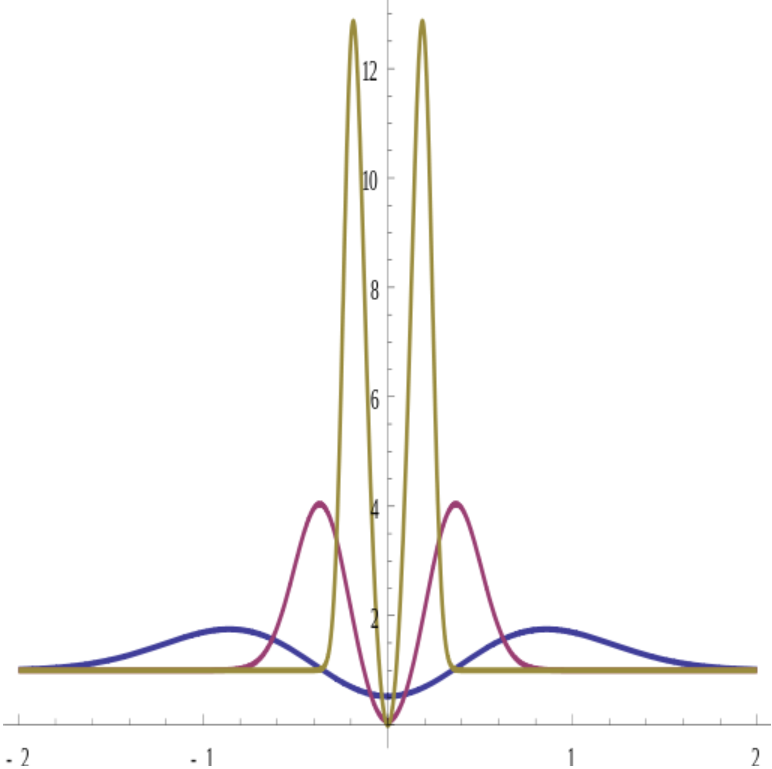
\includegraphics[width=.5\textwidth]{./Hodges-estimator-risk-function.png}
\caption{The mean square error (times n) of Hodges' estimator as a function of \(\mu\). Blue curve corresponds to \(n = 5\), purple to \(n = 50\), and olive to \(n = 500\).}
\end{figure}
\end{frame}


\begin{frame}[label={sec:orgc120596}]{Data-adaptive estimators and irregular estimators}
\begin{equation*}
  \hat{\mu}_n = 
    \begin{cases}
      \hat{X}_n & \text{if } |\hat{X}_n| > n^{-1/4} \\
      0 & \text{if } |\hat{X}_n| \leq n^{-1/4}
    \end{cases}.
\end{equation*}

\vfill

Think of the Hodges' estimator as a \emph{data-adaptive estimator} that work in two
steps:
\begin{enumerate}
\item Conduct a test for whether the mean is 0.
\item If we accept, return 0, otherwise return the empirical average.
\end{enumerate}

\vfill

\cite{leeb2005model} argues that post-model selection estimators are versions of
Hodges' estimator.
\end{frame}

\begin{frame}[label={sec:org0b99517}]{Revisit (annoying) regularity condition}
Asymptotic linearity is easy to motivate. Regularity not so much: ``Why should we
care about data coming from a local perturbation -- we usually just assume that
data are iid.\space{}from some fixed \(P\)?'' \ldots{} 

\vfill


\begin{onlyenv}<1>
\begin{center}

\includegraphics[width=0.7\textwidth]{./sweep-carpet.png}
\end{center}
\end{onlyenv}

\begin{onlyenv}<2>
\begin{center}
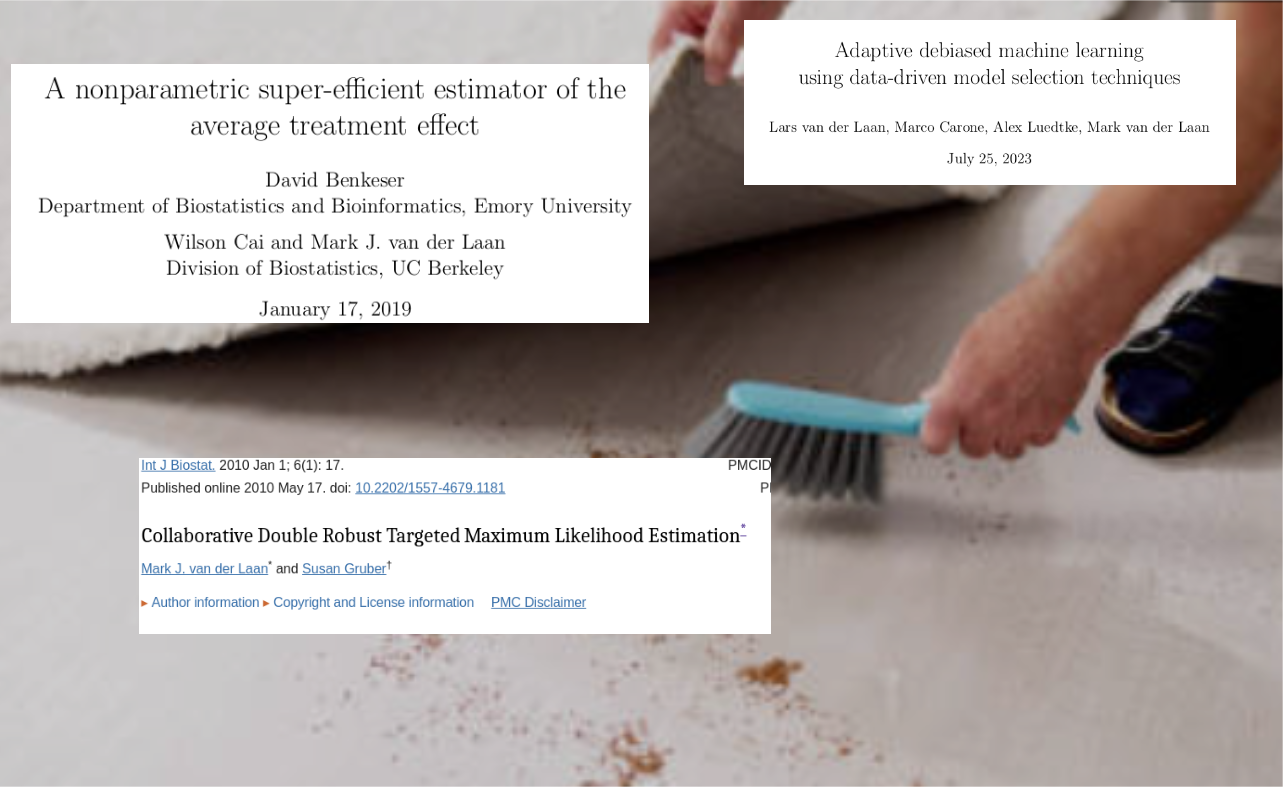
\includegraphics[width=0.7\textwidth]{./sweep-carpet2.png}
\end{center}
\end{onlyenv}
\end{frame}


\begin{frame}[label={sec:orgab9a870}]{Quotes about regularity}
\small

\begin{quote} %% 
Although super-efficient estimators exist, they are unnatural and have undesirable
local properties associated with them. [\ldots{}] From now on, we will restrict
ourselves to regular estimators. \flushright \cite{tsiatis2007semiparametric}
\end{quote}

\begin{quote} %% 
This type of regularity is common and is often considered desirable: A small
change in the parameter should not change the distribution of the estimator too
much; a disappearing small change should not change the (limit) distribution at
all. However, some estimator sequences of interest, such as shrinkage
estimators, are not regular. \flushright \cite{van2000asymptotic}
\end{quote}

\begin{quote} %% 
[\ldots{}] the suggested estimator [\ldots{}] will -- although being consistent -- not be
close to the finite-sample distribution uniformly in the unknown parameters,
thus providing a rather useless estimator. \flushright \cite{leeb2005model}
\end{quote}

\begin{quote} %% 
Such criticisms of superefficient estimators may not be as applicable in
situations in which regular nonparametric estimators do not exist or are too
variable for reliable inference. \flushright \cite{van2023adaptive}
\end{quote}
\end{frame}

\begin{frame}[label={sec:orgb66bb66}]{\color{white} breaker}
\huge\centering \color{bblue} Back to the paper
\end{frame}

\begin{frame}[label={sec:orgb2ca746}]{ADMLE -- the central idea}
Let \(\Psi\) be a target parameter defined on a collection of probability measures
\(\mathcal{M}\).

\vfill

We assume that \(P_0 \in \mathcal{M}_0\) for some \emph{oracle submodel} \(\mathcal{M}_0 \subset \mathcal{M}\), but we don't know \(\mathcal{M}_0\).

\vfill

Estimate the submodel \(\mathcal{M}_0\) from data with \(\mathcal{M}_n\) and
define a projected target parameter \(\Psi_n\) data-adaptively using \(\mathcal{M}_n\).

\vfill

Construct an efficient estimator of the data-adaptive parameter \(\Psi_n\).

\vfill

If \(\mathcal{M}_0\) is much smaller than \(\mathcal{M}\) we expect a
sizable decrease in variance.
\end{frame}

\begin{frame}[label={sec:org5495f19}]{Example of oracle model}

Assume that the data is \( X = (Y, A, W) \) and that we want to estimate the
average treatment effect
\begin{equation*}
  \Psi(P) = \E_P{\left[ \E_P{\left[Y \mid A=1, W \right]} - \E_P{\left[Y \mid A=0, W \right]} \right]}
\end{equation*}

\vfill

An oracle model could be
\begin{equation*}
  \mathcal{M}_0 =
  \begin{Bmatrix}
          \E_P{\left[Y \mid A=a, W=w \right]}
    = \alpha a + \beta^T w
    : \alpha \in \R, \beta \in \R^d,
     \\
    P(\diff a, \diff w) \text{ unspecified}
  \end{Bmatrix}
\end{equation*}

\vfill

Important point is that we do not assume a known model \( \mathcal{M}_0 \),
but only that assume that the data-generating distribution \( P_0 \) actually
belongs to some (unknown) smaller model
\( \mathcal{M}_0 \subset \mathcal{M} \).
\end{frame}


\begin{frame}[label={sec:orgf97d019}]{ADMLE -- more formally}
\begin{enumerate}
\item Specify data-adaptive working models \(\mathcal{M}_n \subset \mathcal{M}\)
intended to approximate \(\mathcal{M}_0\).
\item For some loss function \(\ell \colon \R^d \times \mathcal{M} \rightarrow \R\), define the projection of \(P\) onto the working model \(\mathcal{M}_n\) as

\begin{equation*}
  \Pi_n(P) = \argmin_{Q \in \mathcal{M}_n}\int \ell(x; Q) P(\diff x).
\end{equation*}
\item Define the data-adaptive target parameter \(\Psi_n = \Psi \circ \Pi_n \colon
   \mathcal{M} \rightarrow \R\).
\item Construct an efficient estimator of \(\Psi_n\).
\end{enumerate}

\vfill

An ADMLE \( \hat{\Psi}_n \) is an estimator that satisfies the asymptotic
expansion
\begin{equation*}
  \hat{\Psi}_n  =  \Psi(P_0) + (\empmeas - P_0){[D_{n,P_0}]} + \smallO_P{(n^{-1/2})}
\end{equation*}
where \( D_{n,P_0} \) is the nonparametric efficient influence function of the
data-adaptive target parameter $\Psi_n$.
\end{frame}

\begin{frame}[label={sec:org71370ff}]{\emph{Data-adaptive} and \emph{oracle} target parameters}
Different target parameters are in play:

\begin{description}
\item[{\(\Psi \colon \mathcal{M} \rightarrow \R\)}] The original target parameter.
\item[{\(\Psi_n = \Psi \circ \Pi_n\)}] Data-adaptive target parameter
\item[{\(\Psi_0 = \Psi \circ \Pi\)}] Oracle project-based target parameter.
\end{description}

\vfill

The operator \(\Pi\) is defined as the projection onto the true (but unknown)
oracle submodel,

\begin{equation*}
  \Pi(P) = \argmin_{Q \in \mathcal{M}_0}\int \ell(x; Q) P(\diff x).
\end{equation*}
\end{frame}

\begin{frame}[label={sec:org9daa758}]{The oracle target parameter}
Model selection is known to produce irregular estimators, even when the model
selection step is consistent \citep{leeb2005model}.

\vfill

\cite{van2023adaptive} circumvent this issue by redefining the target to be the
\emph{oracle target parameter} \(\Psi_0 = \Psi \circ \Pi\).

\vfill

While an ADMLE is irregular for the original parameter \(\Psi\), they show that it
is RAL for \(\Psi_0\) (at any \(P_0 \in \mathcal{M}_0\)).

\vfill

\(\Psi_0\) is involves the projection onto the \emph{unknown} oracle model \(\mathcal{M}_0\). If we don't know \(\mathcal{M}_0\) we don't really know
\(\Psi_0\) -- is that weird?

\vfill

Maybe not if we accept that we are trying to ``learn what can be learned'' from
the data.
\end{frame}

\begin{frame}[label={sec:orga5820ca}]{One of the main results}
\begin{theorem}[Theorem 5]
Suppose that the working model \(\mathcal{M}_n\) approximates \(\mathcal{M}_0\) fast enough (sort of like at \(\approx n^{-1/4}\) rate) and that additional
regularity conditions hold. Then, the ADMLE \(\hat{\Psi}_n\) is a \(P_0\)-asymptotically linear estimator for \(\Psi_0\) with influence function equal to
the efficient influence function of \(\Psi_0 \colon \mathcal{M}_{\mathrm{np}}
\rightarrow \R\) at \(P_0\) relative to the nonparametric model \(\mathcal{M}_{\mathrm{np}}\).

\vspace{.5cm}
\end{theorem}

\begin{quote} %% 
\small

An important consequence of Theorem 5 is that an ADMLE is a \(P_0\)-regular
estimator for \(\Psi_0\) relative to the nonparametric model \(\mathcal{M}\).
Hence, even under sampling from a worst-case local perturbation of \(P_0\), an
ADMLE allows locally uniformly valid nonparametric inference on the oracle
parameter \(\Psi_0\). This implies that, at least in a local asymptotic sense,
there is no loss in performance of the ADMLE from empirically learning \(\mathcal{M}_0\) compared to the oracle that knows \(\mathcal{M}_0\) or
\(\Psi_0\).

\flushright \cite{van2023adaptive}
\end{quote}
\end{frame}

\begin{frame}[label={sec:orge1ac269}]{The estimator -- details are lacking}
\begin{quote} %% 

Formally, an ADMLE \( \hat{\Psi}_n \) is an estimator that satisfies the
asymptotic expansion
\begin{equation*}
  \hat{\Psi}_n  =  \Psi(P_0) + (\empmeas - P_0){[D_{n,P_0}]} + \smallO_P{(n^{-1/2})}
\end{equation*}
where \( D_{n,P_0} \) is the nonparametric efficient influence function of
$\Psi_n$.

\flushright \cite{van2023adaptive}

\vfill
\end{quote}

\begin{block}{}
Not so clear how to implement an ADML in practice. Example with relaxed lasso
in + standard model robust sandwich estimator of the variance.
\end{block}
\end{frame}

\begin{frame}[label={sec:orgfd6327a}]{Model selection}
\begin{quote} %% 
Suppose that we can employ data-driven model selection techniques to learn a
working statistical model \(\mathcal{M}_n \subset \mathcal{M}\) that sufficiently
approximates some unknown submodel \(\mathcal{M}_0 \subset \mathcal{M}\). Although
the working model \(\mathcal{M}_n\) may not contain the true data-generating
distribution \(P_0\) for any \(n\), we assume that \(\mathcal{M}_0\) is a
smooth statistical model containing \(P_0\). The smoothness condition on \(\mathcal{M}_0\) rules out degenerate models such as \(\mathcal{M}_0 = \{P_0\}\).

\flushright \cite{van2023adaptive}
\end{quote}

\begin{block}{}
When to stop? How do we make sure not to be to aggressive in the model selection
step? Nor to conservative?

\hfill

What to do if we are willing to accept an approximate model \(\mathcal{M}_n\)
that does not contain \(P_0\)?

\hfill

For any \(P_0\) there are many smooth models (nested and non-nested) which can
be assumed to contain \(P_0\).
\end{block}
\end{frame}


\begin{frame}[label={sec:orgfa4d9a4}]{What is the cost of giving up regularity?}
Imposing a smaller submodel \(\mathcal{M}_0\) can introduce bias but reduces
variance \(\rightarrow\) classic bias-variance trade-off.

\vfill

Working with the projection-based oracle parameter \(\Psi_0\) brings the deal back
to a classic bias-variance trade-off.

\vfill

If we consider the original target parameter \(\Psi\), the ADMLE will be irregular
\(\rightarrow\) here we are trading variance for something else -- irregularity.

\vfill

\begin{quote} %% 
Sacrificing some regularity can be justifiable to achieve efficiency gains,
especially when nonparametric regular estimators for \(\Psi\) are unavailable,
such as when the ATE is nonparametrically unidentifiable.

\flushright \cite{van2023adaptive}
\end{quote}

\begin{block}{}
What is the cost? What deal are we making?
\end{block}
\end{frame}

\begin{frame}[label={sec:org59729cc}]{Is regularity a binary concept?}
\begin{theorem}[Theorem 6]

... $\hat{\Psi}_n$ (the ADMLE) is \( P_0 \)-regular for $\Psi$ (the original
target parameter) over all local alternatives \( P_{0,h n^{-1/2}} \) in the
oracle submodel \( \mathcal{M}_0 \). Consequently,
\( \sqrt{n}(\hat{\Psi}_n-\Psi_0) \rightsquigarrow \mathcal{N}(0,
\V{[D_{0,P_0}(O)]}) \), even under sampling from local perturbations of
\( P_0 \) remaining in \( \mathcal{M}_0 \).

\hfill
\end{theorem}

\begin{quote} %% 
Theorem 6 shows that the regularity and superefficiency of ADMLEs fall in a
continuous spectrum driven by the size of the oracle model.

\flushright \cite{van2023adaptive}
\end{quote}

\begin{block}{}
Maybe Hodge's estimator is extreme with \(\mathcal{M}_0 = \{P_0\}\). Can we
expect less irregularity if \(\mathcal{M}_0\) is large? Could it be OK to give
up some regularity, i.e., not be stable under all local perturbations but under
some?
\end{block}
\end{frame}


\begin{frame}[label={sec:org7986a3d}]{Conclusions}
\begin{itemize}
\item It might be ``asymptopia'' to say that we estimate ATE in the non-parametric
model when we have high-dimensional longitudinal data.
\item Sometimes we will be forced to impose restrictions/constraints to make things
work in practice (and maybe even in theory).
\item Can we ask the data how complex the questions we ask can be?
\item Is it a good idea to try to automate an formalize this process -- or should we
just work heuristically?
\item Should we be willing to give up (some degree of) regularity?
\end{itemize}
\end{frame}


\begin{frame}[label={sec:orgbd24ed4}]{References}
\footnotesize \bibliography{bib.bib}
\end{frame}
\end{document}